\cchapter{مقدمه}
مسائل بازیابی تخصص به برسی و تحلیل میزان تخصص افراد، حوزه های فعالت آن ها و همچنین میزان عمیق بودن آن ها در هر حوضه تخصص می پردازد.
\\
مطالعات پیشن در این حوزه به معرفی روش هایی میپردازد که با تحلیل متن هایی که هر کاربر در یک سری از وب سایت های مرتبط تولید کرده است . تخصص های آن کاربر را مشخص کرده و با تکنیک های خوشه بندی این مهارت ها را به دسته های مشخص تقسیم بندی میکند.
از طرف دیگر مطالعاتی وجود دارد که میزان عمق دانش کاربران در هر حوزه تخصصی را مشخص میکند. و به این صورت مشخص میکند که کاربر از لحاظ میزان مهارت در حد یک کارآموز میباشد یا مهارت های عمیق تری دارد و میتوان آن را در سطوخ بالاتر قرار داد.
\\
در این مطلب تلاش شده در ادامه مطالعات پیشین روش هایی ارائه شود که از طریق آن با برسی تغییرات تخصص افراد در حوزه های مختلف پیش بینی از تخصص هایی که فرد احتمالا در آینده یه سراغ آن ها خواهد رفت ارائه کند.
این موضوع از چند جهت حائز اهمیت است. اول این که کسب و کار هایی که به دنبال جذب نیروی کارآموز و آموزش آن میباشند میتوانند با این تکنیک ها مسیر پیش بینی شده آینده آن فرد را پیدا کرده و از میان کاندید های موجود فردی را که مسیر یادگیری مهارت او تناسب بیشتری با نقشه راهی که آن کسب و کار برای آینده آن کارآموز در نظر گرفته مطابقت دارد جذب میکند.
\\
از جهت دیگر کسب و کار هایی که در نقشه راه آن ها بگونه ای است که در ماه ها و سال های آینده به سراغ یک تکنولوژی یا ابزار خاص خواهند رفت نیازی نیست که از ماه ها قبل فردی را با آن مهارت جذب کنند (این کار هزینه بالاتری برای کسب و کار دارد).  آن ها با استفاده از این تکنیک فردی را که مهارت استفاده از ابزار هایی را دارد که کسب و کار در حال حاضر از آن استفاده میکند را دارد و پیشبینی مسیر یادگیری او به گونه ای است که در آینده در مهارتی که به کسب و کار اضافه میشود تخصص پیدا میکنند جذب میکند.
\\
علاوه بر دو مثال فوق میتوان مثال های دیگری نیز ارائه کرد که این راهکار فرآیند جذب و استخدام را بهینه میکند و هزینه نهایی آموزش نیروی جدید را برای کسب و کار ها کاهش میدهد.
\cite{retrival}

\cchapter{ادبیات تحقیق}

\section{مدل های احتمالاتی}
\hspace*{2em}
مدل‌های احتمالاتی به منظور تحلیل و پیش‌بینی پدیده‌ها و داده‌ها با استفاده از اصول احتمال به	 کار می‌روند. این مدل‌ها از مفاهیم احتمالات برای مدل‌سازی عدم قطعیت و تغییرپذیری داده‌ها بهره می‌برند. از جمله کاربردهای مدل‌های احتمالاتی می‌توان به تشخیص الگوها، پیش‌بینی نتایج و تصمیم‌گیری تحت عدم قطعیت اشاره کرد. این مدل‌ها در زمینه‌های مختلف مانند یادگیری ماشین، پردازش زبان طبیعی و تحلیل داده کاربرد دارند. با استفاده از داده‌های تاریخی و توزیع‌های احتمالی، مدل‌های احتمالاتی می‌توانند نتایج آینده را با دقت بالاتری پیش‌بینی کنند.

\section{خوشه بندی}
\hspace*{2em}
خوشه‌بندی به‌عنوان یکی از تکنیک‌های مهم در حوزه بازیابی اطلاعات و به‌ویژه در بازیابی تخصص‌ها نقش 	بسزایی ایفا می‌کند. خوشه‌بندی فرآیندی است که طی آن، مجموعه‌ای از داده‌ها به گروه‌های مشابه و همگن تقسیم می‌شوند. این تکنیک با هدف دسته‌بندی داده‌ها به گونه‌ای انجام می‌شود که داده‌های موجود در هر خوشه بیشترین شباهت را به یکدیگر و کمترین شباهت را به داده‌های خوشه‌های دیگر داشته باشند.
\\
در حوزه بازیابی تخصص‌ها، خوشه‌بندی می‌تواند برای شناسایی و گروه‌بندی تخصص‌های مشابه استفاده شود. به‌طور مثال، می‌توان متخصصانی که در یک زمینه خاص فعالیت دارند را در یک خوشه قرار داد تا به این ترتیب، بازیابی اطلاعات مرتبط با تخصص‌ها به شکل کارآمدتر و دقیق‌تری انجام شود. این امر می‌تواند در سیستم‌های پیشنهاددهنده، جستجوهای تخصصی و تحلیل شبکه‌های اجتماعی به کار رود.
\\
روش‌های مختلفی برای انجام خوشه‌بندی وجود دارد که از جمله مهم‌ترین آن‌ها می‌توان به روش‌های مبتنی بر فاصله، و روش‌های سلسله‌مراتبی اشاره کرد. هر یک از این روش‌ها با توجه به ویژگی‌های داده‌ها و اهداف خوشه‌بندی، مزایا و محدودیت‌های خاص خود را دارند.
\\
در حوزه بازیابی اطلاعات، خوشه‌بندی علاوه بر دسته‌بندی تخصص‌ها، می‌تواند به بهبود دقت نتایج جستجو، کاهش پیچیدگی فضای جستجو و افزایش کارایی سیستم‌های بازیابی کمک کند. به‌عنوان مثال، با خوشه‌بندی مدارک و مقالات علمی، می‌توان به جستجوی موضوعات مرتبط پرداخت و نتایج دقیق‌تری را به کاربران ارائه داد.
\\
در نهایت، می‌توان گفت که خوشه‌بندی به‌عنوان یکی از ابزارهای قدرتمند در تحلیل داده‌ها و بازیابی اطلاعات، نقش کلیدی در بهبود فرآیندهای بازیابی تخصص‌ها و مدیریت دانش ایفا می‌کند و می‌تواند به ارتقای سطح کیفی سیستم‌های اطلاعاتی منجر شود.

\section{مدل‌های احتمالاتی بر پایه پیش‌بینی آینده}
\hspace*{2em}
این مدل‌ها بر پایه تئوری احتمال و آمار بنا شده‌اند و با استفاده از داده‌های گذشته، سعی در پیش‌بینی وقایع و روندهای آینده	  دارند. در بازیابی تخصص‌ها، مدل‌های احتمالاتی می‌توانند برای پیش‌بینی نیازهای آینده به تخصص‌های خاص، شناسایی تغییرات در الگوهای تخصص و پیشنهاد تخصص‌های مورد نیاز در بازار کار استفاده شوند .یکی از کاربردهای مهم مدل‌های احتمالاتی در بازیابی تخصص‌ها، تحلیل پیش‌بینانه بر اساس داده‌های تاریخی است. این مدل‌ها با تحلیل داده‌های مربوط به فعالیت‌های گذشته متخصصان و روندهای شغلی، می‌توانند پیش‌بینی‌هایی در مورد آینده این تخصص‌ها ارائه دهند. به‌عنوان مثال، با استفاده از مدل‌های احتمالاتی می‌توان تخصص‌هایی که احتمال رشد بالایی دارند را شناسایی کرده و به کاربران پیشنهاد داد.
\\
از جمله روش‌های معروف در این حوزه، مدل‌های مارکوف، زنجیره‌های زمانی و تحلیل رگرسیون می‌باشند. مدل‌های مارکوف با استفاده از احتمال انتقال از یک حالت به حالت دیگر، روندهای آینده را پیش‌بینی می‌کنند. زنجیره‌های زمانی نیز با تحلیل داده‌های سری زمانی و بررسی الگوهای تکرار شونده، به پیش‌بینی آینده می‌پردازند. تحلیل رگرسیون نیز با استفاده از متغیرهای مستقل و وابسته، روابط بین داده‌ها را مدل‌سازی کرده و پیش‌بینی‌های دقیقی ارائه می‌دهد.
\\
این مدل‌ها نه تنها در پیش‌بینی روندهای آینده، بلکه در بهبود سیستم‌های پیشنهاددهنده و جستجو نیز کاربرد دارند. به‌طور مثال، با پیش‌بینی نیازهای آینده به تخصص‌های خاص، سیستم‌های بازیابی می‌توانند به کاربران خود تخصص‌های مورد نیاز در آینده را پیشنهاد دهند و آن‌ها را برای بازار کار آینده آماده کنند.
\\
در مجموع، مدل‌های احتمالاتی با توانایی پیش‌بینی و تحلیل داده‌ها، نقش کلیدی در بهبود کارایی سیستم‌های بازیابی اطلاعات و تخصص‌ها ایفا می‌کنند و به بهینه‌سازی فرآیندهای تصمیم‌گیری و مدیریت دانش کمک می‌نمایند.

\section{یادگیری ماشین}
\hspace*{2em}
یادگیری ماشین به عنوان یکی از شاخه‌های پیشرفته و نوین علوم کامپیوتر، در سال‌های اخیر مورد توجه فراوانی قرار گرفته است. این فناوری با استفاده از الگوریتم‌ها و مدل‌های ریاضی قادر است به تحلیل و تفسیر داده‌ها پرداخته و الگوهای موجود در آنها را شناسایی کند. یکی از کاربردهای مهم یادگیری ماشین، پیش‌بینی آینده بر اساس داده‌های گذشته و حال است. در زمینه بازیابی اطلاعات، یادگیری ماشین می‌تواند نقش مؤثری در بهبود فرآیند بازیابی تخصص‌ها ایفا کند. بازیابی تخصص‌ها، که زیرمجموعه‌ای از بازیابی اطلاعات محسوب می‌شود، به معنای شناسایی و استخراج دانش و مهارت‌های افراد متخصص در یک حوزه خاص است.
\\
با استفاده از تکنیک‌های یادگیری ماشین، می‌توان الگوها و روابط پنهان میان داده‌های موجود را شناسایی و از آنها برای پیش‌بینی تخصص‌ها و مهارت‌های مورد نیاز در آینده استفاده کرد. مدل‌های یادگیری ماشین قادرند با تحلیل داده‌های مربوط به سوابق کاری، مقالات علمی، پروژه‌های تحقیقاتی و سایر منابع مرتبط، به شناسایی الگوهای تخصصی بپردازند. این مدل‌ها می‌توانند بر اساس داده‌های جمع‌آوری شده، نیازهای آتی بازار کار را پیش‌بینی کرده و به سازمان‌ها کمک کنند تا برای آینده آماده باشند. به عنوان مثال، با تحلیل داده‌های موجود، می‌توان پیش‌بینی کرد که کدام تخصص‌ها در سال‌های آتی بیشتر مورد نیاز خواهند بود و چه مهارت‌هایی باید تقویت شوند. به طور خلاصه، یادگیری ماشین با توانایی پیش‌بینی آینده و تحلیل داده‌های موجود، می‌تواند به عنوان ابزاری قدرتمند در بهبود فرآیند بازیابی تخصص‌ها و افزایش کارایی سازمان‌ها و نهادها عمل کند. این فناوری نه تنها به شناسایی تخصص‌های مورد نیاز کمک می‌کند، بلکه می‌تواند به توسعه و بهبود مهارت‌های فعلی نیز یاری رساند.

\section{بازیابی سند}
\hspace*{2em}
بازیابی سند به عنوان بخشی اساسی از علم اطلاعات، نقش مهمی در پژوهش‌های ادبیات موضوعی ایفا می‌کند. این فرآیند به معنای جستجو، انتخاب و بازیابی مستندات و اسناد مرتبط با یک موضوع خاص است. با استفاده از روش‌های پیشرفته بازیابی اطلاعات، می‌توان الگوها و روابط پنهان در بین متون ادبی را شناسایی کرده و به تحلیل دقیق‌تری از آنها پرداخت. بازیابی سند با استفاده از فنون یادگیری ماشین و پردازش زبان طبیعی، می‌تواند به پیش‌بینی موضوعات و مسائل آینده در ادبیات موضوعی کمک کند. این روش‌ها با تجزیه و تحلیل متون موجود، می‌توانند الگوهایی را کشف کنند که در آینده به عنوان موضوعات جدید یا جنبه‌های نو ادبیات مطرح خواهند شد. به طور خلاصه، بازیابی سند با بهره‌گیری از رویکردهای پیشرفته علم اطلاعات و همچنین فنون یادگیری ماشین، می‌تواند در پژوهش‌های ادبیات موضوعی به بهبود فرآیند انتخاب و تحلیل متون کمک کند و به پیش‌بینی آینده این حوزه نیز کمک نماید.


\section{سری های زمانی}
\hspace*{2em}

سری‌های زمانی به عنوان یک روش تحلیلی در علوم داده‌ها، برای مدل‌سازی و پیش‌بینی رفتار آینده داده‌ها استفاده می‌شوند. این روش بر مبنای مشاهدات متوالی در طول زمان استوار است که می‌تواند شامل داده‌های مالی، آب و هوا، فروش و غیره باشد. هدف اصلی تحلیل سری‌های زمانی، شناسایی الگوها و روندهای موجود در داده‌ها و استفاده از آنها برای پیش‌بینی مقادیر آینده است. در تحلیل سری‌های زمانی، مفاهیم اساسی شامل روند، فصلی بودن و نویز هستند. روند به تغییرات بلندمدت در داده‌ها اشاره دارد، در حالی که فصلی بودن به الگوهای تکراری در بازه‌های زمانی مشخص اطلاق می‌شود. نویز نیز به نوسانات تصادفی و غیرقابل پیش‌بینی در داده‌ها گفته می‌شود. 
یکی از روش‌های متداول برای مدل‌سازی سری‌های زمانی، مدل‌های خودهمبستگی و میانگین متحرک است. در این مدل‌ها، مقادیر آینده به صورت تابعی از مقادیر گذشته و خطاهای پیش‌بینی قبلی تخمین زده می‌شوند. به عنوان مثال، مدل‌های خودهمبستگی مقادیر آینده را بر اساس همبستگی مقادیر گذشته پیش‌بینی می‌کنند، در حالی که مدل‌های میانگین متحرک از خطاهای پیش‌بینی‌های قبلی برای اصلاح مقادیر آینده استفاده می‌کنند. روش دیگر برای تحلیل سری‌های زمانی، تحلیل طیفی است که در آن سری‌های زمانی به اجزای فرکانسی تجزیه می‌شوند. این روش برای شناسایی دوره‌های مختلف نوسانات در داده‌ها مفید است.
\\
در حوزه بازیابی تخصص‌ها، تحلیل سری‌های زمانی می‌تواند به پیش‌بینی نیازهای آتی بازار کار و تخصص‌های مورد نیاز کمک کند. با تحلیل داده‌های تاریخی مربوط به استخدام‌ها، پروژه‌ها و مهارت‌های مورد تقاضا، می‌توان روندهای تغییرات در بازار کار را شناسایی کرده و برای برنامه‌ریزی‌های آتی استفاده کرد. به طور خلاصه، تحلیل سری‌های زمانی با شناسایی الگوها و روندهای موجود در داده‌ها، ابزاری قدرتمند برای پیش‌بینی آینده و تصمیم‌گیری‌های مبتنی بر داده فراهم می‌کند. این روش به ویژه در حوزه‌هایی که نیاز به پیش‌بینی دقیق و برنامه‌ریزی بلندمدت دارند، کاربرد دارد.


\section{معیار های ارزیابی}
\hspace*{2em}
ارزیابی مدل‌های بازیابی اطلاعات در حوزه علوم کامپیوتر با استفاده از معیارهای مختلفی مانند دقت، بازآوری و میانگین دقت متوسط (MAP) انجام می‌شود که هر یک از این معیارها جنبه‌های متفاوتی از عملکرد مدل را اندازه‌گیری می‌کنند.

دقت (Precision) به معنای نسبت تعداد مدارک مرتبط بازیابی‌شده به کل مدارک بازیابی‌شده است. به بیان دیگر، دقت نشان می‌دهد که از میان مدارکی که توسط مدل بازیابی شده‌اند، چند درصد از آن‌ها واقعاً مرتبط با پرسش کاربر بوده‌اند. به عنوان مثال، اگر مدل ۱۰ مدرک را بازیابی کند و از این تعداد، ۷ مدرک مرتبط باشند، دقت مدل ۷۰ درصد خواهد بود. دقت بالا نشان می‌دهد که مدل قادر است نتایج دقیق‌تری را به کاربر ارائه دهد و خطای نوع اول (False Positive) کمتر است.
\\
بازآوری (Recall) معیار دیگری است که تمرکز آن بر میزان بازیابی مدارک مرتبط است. بازآوری به معنای نسبت تعداد مدارک مرتبط بازیابی‌شده به کل مدارک مرتبط موجود در مجموعه است. به عبارت دیگر، این معیار نشان می‌دهد که مدل تا چه حد توانسته است تمامی مدارک مرتبط با پرسش کاربر را بازیابی کند. برای مثال، اگر در مجموعه ۲۰ مدرک مرتبط وجود داشته باشد و مدل ۱۵ مورد از آن‌ها را بازیابی کند، بازآوری ۷۵ درصد خواهد بود. بازآوری بالا نشان‌دهنده توانایی مدل در یافتن اکثر یا تمامی مدارک مرتبط است و نشان می‌دهد که خطای نوع دوم (False Negative) کمتر است.
\\
میانگین دقت متوسط (MAP) یکی از جامع‌ترین معیارها برای ارزیابی مدل‌های بازیابی اطلاعات است که هر دو جنبه دقت و بازآوری را در نظر می‌گیرد. MAP به این صورت محاسبه می‌شود که ابتدا برای هر پرسش دقت در هر رتبه‌ای که یک مدرک مرتبط بازیابی می‌شود محاسبه می‌گردد. سپس دقت‌های میانگین برای هر پرسش محاسبه شده و در نهایت میانگین این دقت‌ها برای تمامی پرسش‌ها به عنوان MAP محاسبه می‌شود.
\\
MAP می‌تواند به عنوان یک معیار کلی برای مقایسه عملکرد مدل‌های مختلف مورد استفاده قرار گیرد، زیرا هم دقت در رتبه‌های بالاتر و هم توانایی مدل در بازیابی مدارک مرتبط در طول تمامی رتبه‌ها را می‌سنجد. به دلیل این ویژگی‌ها، MAP اغلب در مقالات علمی و ارزیابی سیستم‌های بازیابی اطلاعات به کار می‌رود.
\\
با استفاده از این معیارها، محققان و مهندسان می‌توانند مدل‌های بازیابی اطلاعات را از جنبه‌های مختلف ارزیابی کرده و نقاط قوت و ضعف هر مدل را شناسایی کنند. این امر به بهبود سیستم‌های بازیابی اطلاعات و ارائه نتایج دقیق‌تر و کامل‌تر به کاربران کمک شایانی می‌کند. به طور کلی، درک صحیح از این معیارها و استفاده مناسب از آن‌ها می‌تواند تأثیر قابل توجهی در طراحی و بهینه‌سازی سیستم‌های بازیابی اطلاعات داشته باشد.


\cchapter{کار های مرتبط}
به طور کلی کار هایی که در حوزه بازیابی تخصص انجام شده را میتوان به چهار دسته کلی تقسیم کرد این چهار دسته شامل موارد زیر میباشد.
\begin{itemize}
	\item شناسایی منابع داده
	\item استخراج داده
	\item طبقه بندی تخصص ها
	\item خودکار سازی فرآیند استخراج و طبقه بندی
\end{itemize}
در این مطلب نتیجه کار های پیشین در دسته سوم یعنی طبقه بندی تخصص ها مورد استفاده قرار گرفته و با استفاده از روش های خوشه بندی که در کار های گذشته معرفی شده، حوزه های مهارتی آینده افراد شناسایی میشود.
در این بخش به توضیح کار های پیشین انجام شده در بخش سوم پرداخته میشود.
\cite{expret}



\section*{طبقه بندی تخصص ها}

در این بخش از پایان‌نامه، مروری بر تحقیقات پیشین در زمینه بازنمایی تخصص انجام شده است. این حوزه با استفاده از تکنیک‌های مختلفی برای استخراج و نمایش تخصص افراد از داده‌های موجود، توسعه یافته است. بر اساس مرور انجام شده، این تحقیقات به سه جنبه اصلی تقسیم می‌شوند: روش‌های بازنمایی، پشتیبانی زمانی، و پشتیبانی معنایی.
\cite{intern}
\cite{tshape}
\subsection*{روش‌های بازنمایی تخصص} روش‌های مختلفی برای بازنمایی تخصص در متون علمی به کار گرفته شده‌اند که هر کدام بر اساس نوع داده‌ها و اهداف خاص تحقیقاتی طراحی شده‌اند. این روش‌ها را می‌توان به پنج دسته اصلی تقسیم کرد: \begin{itemize} \item \textbf{فراوانی اصطلاحات:} این روش بر مبنای تعداد دفعات تکرار اصطلاحات در متون علمی استوار است. در این رویکرد، هر واژه به عنوان یک بُعد در نظر گرفته می‌شود و بر اساس تعداد تکرار آن در متن، میزان تخصص فرد یا ارتباط متن با یک موضوع خاص ارزیابی می‌شود. \item \textbf{مدل‌های زبانی:} این مدل‌ها با استفاده از تحلیل احتمالی توزیع واژه‌ها در متون، یک مدل زبانی ایجاد می‌کنند که می‌تواند برای ارزیابی میزان شباهت متون جدید با متون قبلی به کار رود. \item \textbf{مدل‌های موضوعی:} این مدل‌ها توزیع احتمالی موضوعات در متون را تحلیل می‌کنند. یکی از معروف‌ترین روش‌ها در این دسته، \lr{Latent Dirichlet Allocation (LDA)} است که برای شناسایی موضوعات اصلی در یک مجموعه داده به کار می‌رود. \item \textbf{گراف:} در این روش، داده‌های تخصص به صورت یک گراف نمایش داده می‌شوند. سپس با استفاده از الگوریتم‌های خاص مانند \lr{PageRank} یا \lr{Random Walk}، روابط و رتبه‌بندی تخصص‌ها تحلیل می‌شود. \item \textbf{روش‌های سفارشی:} این دسته شامل رویکردهای خاصی است که در آن‌ها از تکنیک‌های جایگزین برای بازنمایی تخصص استفاده می‌شود. به عنوان مثال، برخی مطالعات از داده‌های باز پیوندی (\lr{LOD}) برای ساخت پروفایل‌های پژوهشگران استفاده می‌کنند. \end{itemize}

\subsection*{پشتیبانی زمانی} تخصص افراد ممکن است با گذر زمان تغییر کند و این تغییرات می‌تواند به دلیل تغییر علاقه‌مندی‌ها یا تغییرات در حوزه‌های تحقیقاتی باشد. بنابراین، در تحلیل تخصص، باید زمان نیز به عنوان یک عامل مهم در نظر گرفته شود. تحقیقات در این زمینه به دو دسته اصلی تقسیم می‌شوند: \begin{itemize} \item \textbf{برش‌های زمانی:} در این رویکرد، تغییرات تخصص در طول زمان به صورت برش‌های زمانی مانند سال بررسی می‌شود. این روش به تحلیل تغییرات تدریجی در تخصص و پیش‌بینی علاقه‌مندی‌های آینده کمک می‌کند. \item \textbf{پیوسته:} این روش‌ها نیازی به برش‌های زمانی مشخص ندارند و تغییرات تخصص را به صورت پیوسته در طول زمان بررسی می‌کنند. این رویکردها با استفاده از برچسب‌های زمانی مرتبط با هر داده، تغییرات در تخصص افراد را تحلیل می‌کنند. \end{itemize}

\subsection*{پشتیبانی معنایی} پشتیبانی معنایی به معنی استفاده از ساختارهای معنایی برای بهبود تحلیل و بازنمایی تخصص است. در حالی که بسیاری از مطالعات موجود از پشتیبانی معنایی استفاده نمی‌کنند، برخی از تحقیقات از هستی‌شناسی‌ها (\lr{Ontology}) و پایگاه‌های دانش (\lr{Knowledge Base}) برای این منظور بهره می‌برند. این ابزارها به تحلیل بهتر مفاهیم موجود در متون و ارتباطات معنایی بین آن‌ها کمک می‌کنند.

\subsection*{خوشه بندی تخصص ها}
در این بخش کارهای پیشین با تمرکز روی تحلیل متن پاسخ کاربران در وبسایت ها سعی در استخراج تخصص آن ها و سپس قرار دادن هر پاسخ در یک حوزه مهارتی میباشد.
همچنین با این روش حوزه های مهارتی افراد شناسایی میشود.

\section*{درخت موضوعی}
در این بخش به توضیح سلسه مراتب موضوعاتی که در این مطلب آمده است و در زمینه آن کارهایی انجام شده است پرداخته میشود.

\subsection*{بازیابی اطلاعات}
والد تمام برگ های درخت موضوعی بازیابی اطلاعات میباشد.
بازیابی اطلاعات یکی از حوزه‌های مهم در علوم کامپیوتر است که به مطالعه روش‌ها و تکنیک‌های جستجو و بازیابی اطلاعات از مجموعه‌های عظیمی از داده‌ها می‌پردازد. با توجه به رشد روزافزون تولید داده، سیستم‌های بازیابی اطلاعات نقش مهمی در ارائه نتایج مرتبط و دقیق به کاربران ایفا می‌کنند. این سیستم‌ها در موتورهای جستجوی وب، پایگاه‌های داده و بسیاری از کاربردهای دیگر مورد استفاده قرار می‌گیرند. مباحث مهم در این حوزه شامل مدل‌های بازیابی، الگوریتم‌های ایندکس‌سازی، پردازش زبان طبیعی و یادگیری ماشین است. چالش‌های اصلی در بازیابی اطلاعات عبارتند از: حجم عظیم داده‌ها، تنوع داده‌ها، ابهام و چند معنایی پرس‌وجوها و تغییرات مداوم در داده‌ها. با مطالعه و بررسی این حوزه، می‌توان راهکارهای نوینی برای بهبود کارایی سیستم‌های جستجو و کشف اطلاعات ارائه داد.

\subsection*{بازیابی تخصص}
بازیابی تخصص فرزند مستقیم بازیابی اطلاعات میباشد. بازیابی تخصص شاخه‌ای از علم اطلاعات است که به یافتن افراد یا منابعی که دارای دانش و مهارت‌های خاص در یک حوزه مشخص هستند، می‌پردازد. با توجه به پیچیدگی روزافزون مسائل و نیاز به متخصصین در حوزه‌های مختلف، بازیابی تخصص به یکی از چالش‌های مهم در سازمان‌ها و جوامع تبدیل شده است.

سیستم‌های بازیابی تخصص با استفاده از تکنیک‌های مختلف مانند پردازش زبان طبیعی، یادگیری ماشین و شبکه‌های اجتماعی، تلاش می‌کنند تا افراد با تخصص مناسب را شناسایی و به یکدیگر متصل کنند. این سیستم‌ها با تحلیل رزومه‌ها، مقالات علمی، پروژه‌ها و سایر اطلاعات مرتبط، پروفایل‌های تخصصی افراد را ایجاد کرده و سپس با توجه به نیازهای یک پروژه یا سوال خاص، افراد مناسب را پیشنهاد می‌دهند.

مباحث مهم در حوزه بازیابی تخصص شامل مدل‌های نمایش دانش، الگوریتم‌های تطبیق، شبکه‌های اجتماعی علمی و ارزیابی سیستم‌های توصیه‌گر است. چالش‌های اصلی در این حوزه عبارتند از: تعریف دقیق تخصص، ابهام در توصیف نیازها، پویایی دانش و مهارت‌ها و حفظ حریم خصوصی اطلاعات شخصی.

\subsection*{طبقه بندی تخصص}
این بخش فرزند مستقیم بازیابی تخصص میباشد که در مقدمه این فصل به آن اشاره شده است.

\subsection*{خوشه بندی}
خوشه‌بندی به منظور گروه‌بندی داده‌های مشابه با یکدیگر به کار می‌رود. در واقع، خوشه‌بندی به دنبال یافتن الگوهای پنهان در داده‌هاست و به این ترتیب، به ما کمک می‌کند تا داده‌های بزرگ و پیچیده را بهتر درک کنیم و از آن‌ها برای تصمیم‌گیری بهتر استفاده کنیم. برای مثال، می‌توانیم از خوشه‌بندی برای دسته‌بندی مشتریان یک فروشگاه بر اساس رفتار خرید آن‌ها استفاده کنیم یا مقالات علمی را بر اساس موضوع آن‌ها گروه‌بندی کنیم.

الگوریتم‌های مختلفی برای خوشه‌بندی وجود دارد که هر کدام برای نوع خاصی از داده‌ها مناسب هستند. از جمله این الگوریتم‌ها می‌توان به k-means، سلسله مراتبی، مبتنی بر چگالی و مبتنی بر مدل اشاره کرد. انتخاب الگوریتم مناسب به عوامل مختلفی مانند نوع داده‌ها، تعداد خوشه‌ها و هدف از خوشه‌بندی بستگی دارد. خوشه‌بندی کاربردهای بسیار گسترده‌ای در حوزه‌های مختلف مانند تجارت، پزشکی، بیوانفورماتیک و علوم اجتماعی دارد.
در این درخت موضوعی خوشه بندی یکی از فرزندان مستقیم بحث طبقه بندی تخصص میباشد.

\subsection*{مدل های احتمالاتی}
 مدل های احتمالاتی نیز فرزند گره بازیابی تخصص میباشند البته این مدل های در حوزه های دیگر نیز کاربرد گسترده دارا میباشند ولی در اینجا کاربرد آن در مباحث مربوط به بازیابی اطلاعات و مخصوصا بازیابی تخصص مد نظر میباشد.


\subsection*{تحلیل زمانی}
.در این حوزه تغییرات داده در طول زمان برسی میشود. این بخش فرزند بخش طبقه بندی تخصص میباشد. به گونه ای که تغییرات تخصص افراد در طول زمان برسی میشود

\subsection*{سری های زمانی}
این سری‌ها داده‌های ساختاریافته‌ای هستند که یکی از مشخصه‌های آن‌ها زمان میباشد. در نتیجه میتوان این داده ها را در محور زمان مرتب سازی و تحلیل کرد.
\begin{figure}[tb]
	\centering
	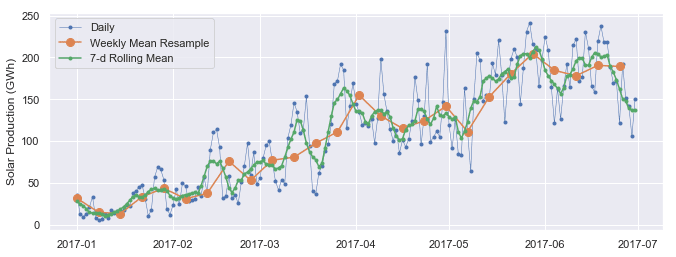
\includegraphics[width=1\linewidth]{time-series-pandas_78_0.png}
	\caption {یک نمونه از سری های زمانی}
	\label{fig:logo}
\end{figure}

\subsection*{پیشبینی آینده}
در این حوزه سعی میشود با تحلیل داده‌های گذشته (معمولا داده های سری های زمانی) تخمین نسبتا دقیقی از آینده ارائه کرد.
روش‌های انجام این پیشبینی معمولا به دو دسته کلی تقسیم میشوند که شامل روش های مبتنی بر یادگیری ماشین و روش های آماری می‌باشد.
هر دو این روش‌ها در حوزه بازیابی تخصص میتوانند مفید واقع شوند ولی به صورت کلی پیاده سازی روش های آماری به مراتب ساده تر از روش های مبتنی بر یادگیری ماشین میباشد.


\subsection*{روش های ارزیابی}
قبل از شروع یافتن روش مناسب برای تخمین تخصص آینده افراد لازم است روشی برای ارزیابی این تخمین وجود داشته باشد.
ساده ترین روش این است که داده‌های مورد آزمون به دو دسته تقسیم شده، دسته قدیمی تر به عنوان داده‌‌هایی برای تخمین و دسته دوم داده هایی هستند که میزان نزدیک بودن تخمین تولید شده از داده ها ی بخش اول میتواند دقت روش را ارزیابی کند.
البته این روش همیشه کارساز نخواهد بود، زیرا در برخی مواقع پس از تخمین داده های جدیدی وجود ندارد که بتوان دقت روش را ارزیابی کرد، در این صورت لازم است از روش های پیچیده تری استفاده شود.

از ساده ترین روش های ارزیابی میتوان سه مورد زیر را نام برد.
\subsubsection*{یادآوری (Recall)}
یادآوری یکی از معیارهای ارزیابی مدل‌های یادگیری ماشین است که به درصد نمونه‌های مثبت درست پیش‌بینی شده نسبت به کل نمونه‌های مثبت اشاره دارد. به عبارت دیگر، یادآوری نشان می‌دهد که مدل تا چه حد قادر است تمام نمونه‌های مثبت موجود در داده‌ها را شناسایی کند. این معیار در کاربردهایی که تشخیص همه موارد مثبت اهمیت دارد، بسیار مهم است؛ مثلاً در شناسایی بیماری‌ها که مهم است هیچ موردی نادیده گرفته نشود. یادآوری بالا نشان‌دهنده این است که مدل موفق به شناسایی تعداد زیادی از نمونه‌های مثبت شده، اما ممکن است برخی از نمونه‌های منفی را به اشتباه مثبت پیش‌بینی کرده باشد. در تعادل میان یادآوری و دقت، افزایش یادآوری معمولاً به کاهش دقت منجر می‌شود. این معیار به ویژه در مسائلی که خطاهای نوع دوم (عدم شناسایی موارد مثبت) حیاتی است، اهمیت دارد.

\subsubsection*{نقشه (MAP)}
 میانگین دقت ترتیبی یک معیار ارزیابی مدل‌های بازیابی اطلاعات و یادگیری ماشین است که کیفیت رتبه‌بندی نتایج را می‌سنجد. این معیار برای مدل‌هایی که چندین خروجی به صورت مرتب شده تولید می‌کنند، اهمیت دارد. نقشه به صورت میانگین دقت در سطوح مختلف رتبه‌بندی محاسبه می‌شود و نشان می‌دهد که نتایج بالاتر رتبه به چه میزان مرتبط هستند. به عبارت دیگر، نقشه به ارزیابی توانایی مدل در مرتب‌سازی صحیح نتایج مرتبط کمک می‌کند. این معیار بیشتر در سیستم‌های پیشنهاددهنده، موتورهای جستجو و کاربردهایی که رتبه‌بندی نتایج اهمیت دارد، استفاده می‌شود. نقشه بالاتر نشان‌دهنده کیفیت بهتر رتبه‌بندی مدل است. این معیار با محاسبه میانگین دقت در هر نقطه که یک نمونه مثبت رتبه‌بندی شده، به دست می‌آید. در نهایت، نقشه ابزاری است برای سنجش کلی عملکرد یک مدل در زمینه رتبه‌بندی.

\subsubsection*{دقت (Precision)}
دقت یکی از معیارهای اساسی ارزیابی مدل‌های یادگیری ماشین است که به نسبت تعداد نمونه‌های مثبت درست پیش‌بینی شده به کل نمونه‌هایی که به عنوان مثبت پیش‌بینی شده‌اند اشاره دارد. به عبارت دیگر، دقت نشان می‌دهد که مدل تا چه حد در پیش‌بینی‌های مثبت خود درست عمل کرده است. دقت بالا به معنای این است که تعداد پیش‌بینی‌های نادرست (مثبت کاذب) کم است و مدل بیشتر بر پیش‌بینی‌های صحیح متمرکز است. این معیار در مواقعی که هزینه اشتباهات مثبت کاذب بالاست، اهمیت ویژه‌ای دارد؛ مثلاً در مواردی که تشخیص اشتباه یک تهدید می‌تواند منجر به اقدامات غیرضروری شود. در مقابل، افزایش دقت معمولاً به کاهش یادآوری منجر می‌شود، زیرا مدل تنها مواردی را به عنوان مثبت پیش‌بینی می‌کند که از صحت آن‌ها مطمئن است. دقت به عنوان یکی از معیارهای مهم در تعیین کارایی مدل‌های یادگیری ماشین شناخته می‌شود و در تعادل با یادآوری به کار می‌رود تا بهترین عملکرد مدل مشخص شود.




\cchapter{نتیجه گیری و کار های آینده}

\section*{ایده و محدوده کاری آینده}
در این موضوع با تحلیل داده های خوشه بندی شده ابتدا یک نمایه از هر کاربر که در فرم های اینترنتی مرتبط فعالیت داشته، ساخته میشود.
این نمایه توصیف میکند که چند درصد فعالیت کاری هر کاربر به یک موضوع خاص اختصاص داده شده است.
سپس یک روش ارزیابی برای امتیازدهی به میزان دقت روش پیشبینی معرفی میشود.
به طور کلی سوالی که مطرح میشود و این مقاله سعی در پاسخ دهی به آن دارد این است که بهترین مدل برای پیشبینی تخصص آینده افراد چه مدلی میباشد. این مدل از میان مدل های یادگیری ماشین یا مدل های آماری انتخاب میشود. برای رسیدن به بهترین مدل ابتدا یک روش مناسب برای ارزیابی دقت مدل معرفی میشود. این روش ارزیابی از میان روش های موجود که چند نمونه آن پیشتر مطرح شد انتخاب میشود. سپس چند مدل کاندید انتخاب شده و پیاده سازی آن انجام خواهد شد و نتیجه خروجی آن توسط روش ارزیابی برسی میشود و بهترین مدل یا چند مدل برتر نسبت به باقی مدل ها معرفی میشود.
پس میتوان خروجی این مقاله را یک مدل معرفی شده در نظر گرفت.
\\
تمام مدل ها با نمونه ای از داده های سایت stackoverflow  آزمون خواهند شد و پیاده سازی هر مدل انجام میشود.
در نتیجه میتوان یک مقایسه میان نتیجه پیشبینی مدل ها روی یک داده ی آزمون انجام داد و از آنجایی که این مقایسه در شرایط برابر میان تمام مدل ها انجام میشود، میتوان نتیجه ارزیابی آن را معتبر درنظر گرفت.
\\
این مقایسه از آنجایی دارای اهمیت است که در صورت یافتن بهترین مدل برای پیشبینی این نوع از داده ها در مرحله اول میتوان از آن مدل در کنار کارهایی که پیشتر انجام شده است، روشی معرفی کرد که نتیجه دقیق تری برای جذب افراد در کسب و کار ها استفاده کرد در مرحله دوم از نتیجه داده های تولید شده در این مطالعه برای مطالعه های آینده استفاده شود.

همچنین کارهایی که در آینده میتوان در ادامه این کار انجام داد شامل معرفی روشی که پیاده سازی این مدل را برای صنعت راحت تر کند و همچنین افزودن متغیر های جدید به مدل آموزش دیده شده برای یافتن نتیجه دقیق‌تر میباشد.



\section*{نتیجه گیری}
به طور کلی مسئله بازیابی نیروی متخصص یک مسئله نسبتا جدید در حوزه بازیابی اطلاعات میباشد. از این رو مسائل باز زیادی همچنان در این حوزه وجود دارد. این مسائل باز بیشتر در حوزه تحلیل داده های استخراج شده، خوشه بندی آن ها و نتیجه گیری از آن‌ها برای یافتن بهترین کاندید یک موقعیت شغلی میباشد.
\\
ضعف اصلی روش های موجود این است که این است که این روش ها معمولا پارامتر های کمی را برای برسی داده های استفاده میکنند و در نتیجه آن خروجی حاصل ممکن است با واقعیت تفاوت داشته باشد.
در سال های اخیر سعی شده با معرفی روش هایی دقت خوشه بندی و تحلیل این داده ها افزایش یابد.
این مطلب نیز سعی در افزایش دقت روش های پیشین با معرفی روشی جدید برای پیشبینی تخصص آینده افراد دارد تا دقت بازیابی تخصص افراد را افزایش دهد.